% !TEX root=/home/tavant/these/manuscript/src/manuscript.tex

\FloatBarrier

\section{Comparison of the sheath model with PIC simulations} \label{subsec-picandmodel}

% \begin{figure}[hbtp]
%   \centering
%   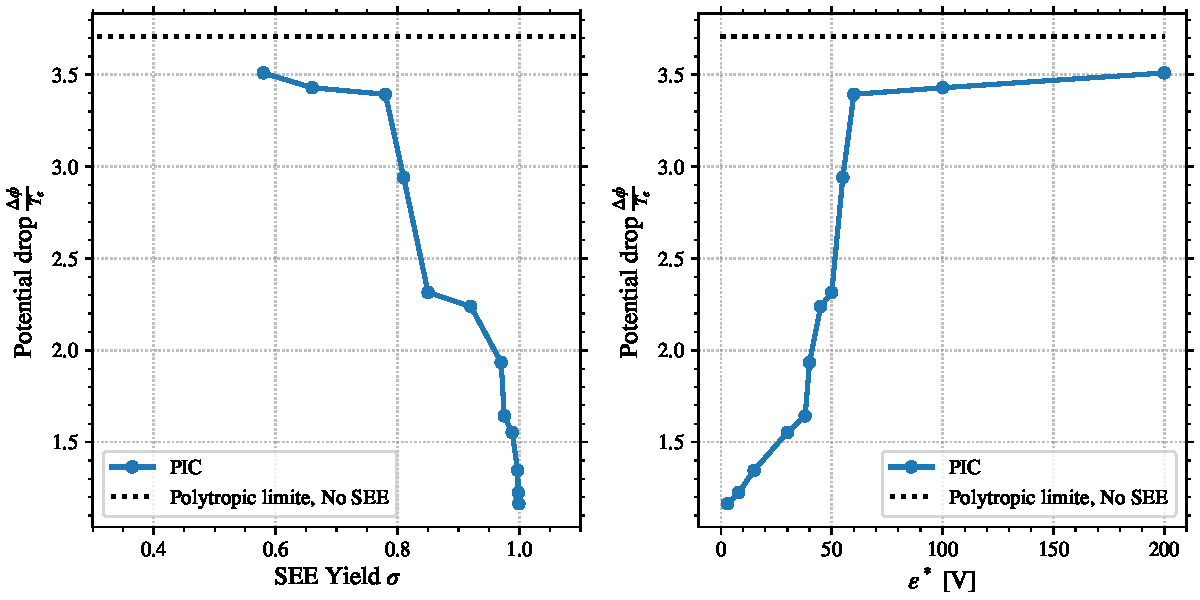
\includegraphics[width=\textwidth]{dphi_polytropic_noSEE}
%   \caption{PIC simulation results (with SEE) compared to the polytropic limit without SEE.}
%   \label{fig-polytropic_pic_noSEE}
% \end{figure}
% 
% \begin{figure}[hbtp]
%   \centering
%   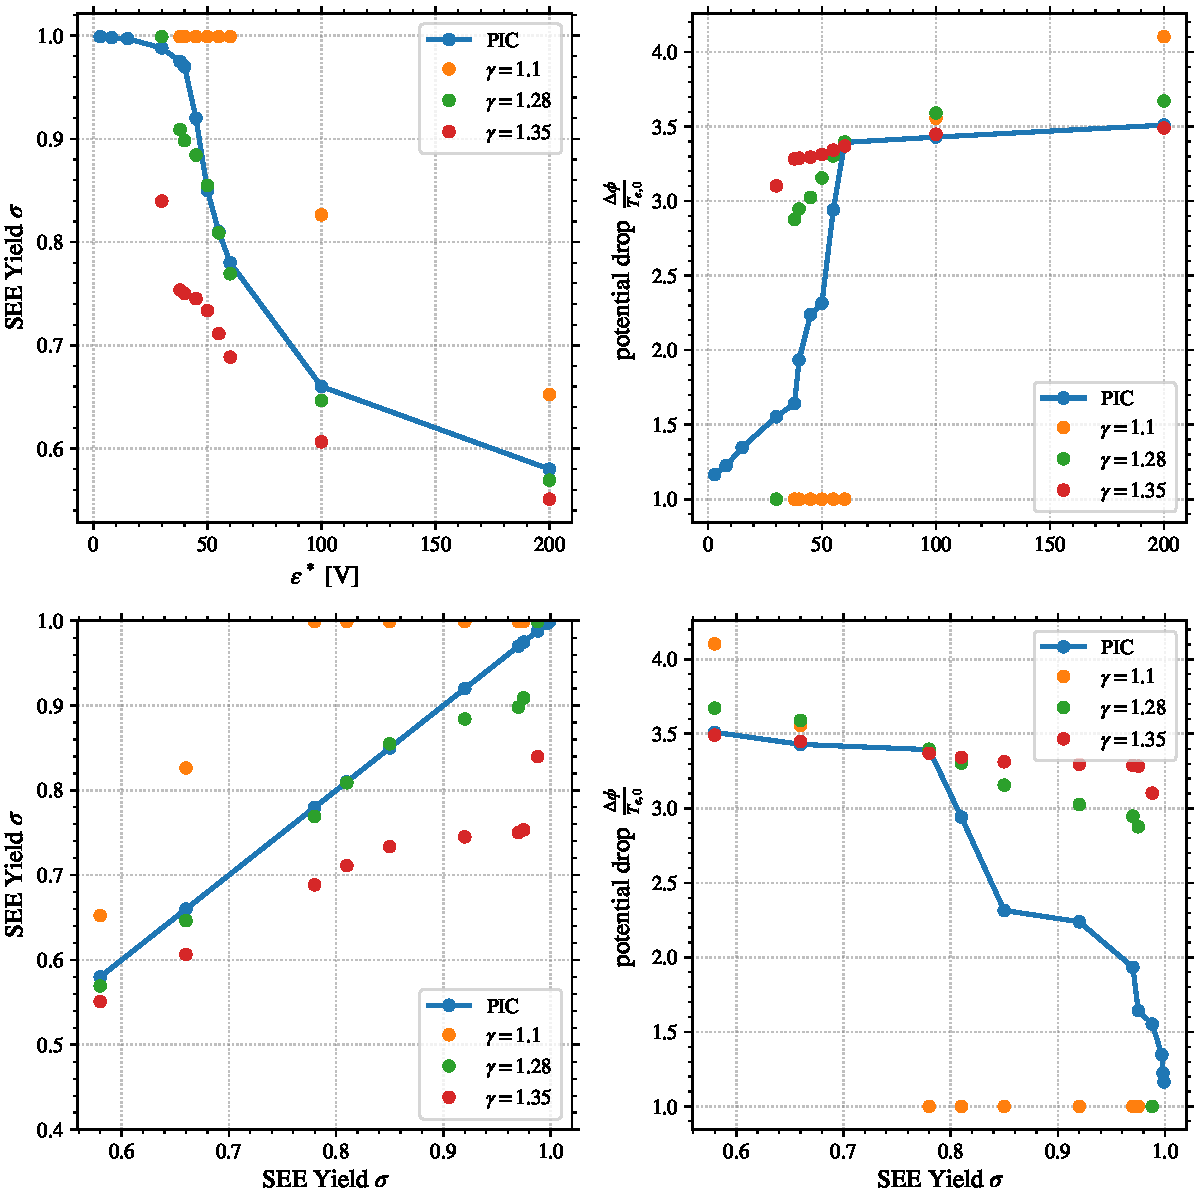
\includegraphics[width=\textwidth]{Summary_polytropic_SEE.pdf}
%   \caption{Comparison of the PIC simulation results with the polytropic model with SEE.}
%   \label{fig-polytropic_see_summary}
% \end{figure}

We compare in this section the characteristics of the plasma wall interaction observed in the \ac{PIC} simulation with the fluid model developed in \cref{sec-fluid_poly_see}.
The variables of interest are the averaged electron emission rate $\rate$ and the plasma potential drop to the wall.
The only input of the model is the electron mean temperature $\Teb$ as well as the polytropic index $\gamma$.
As seen in \cref{sec-PIC_poly}, the polytropic index of the electron population is measured in the \ac{PIC} simulation to $\gamma=1.35$.
However, the electrons going toward the wall present a different index, measured from the bulk \ac{EVDF} to $\gamma=1.28$.
These two values will be compared.
